\chapter{Appendix E: Configuration Verification Screenshots}
\label{app:config-verify}

\section{EoR-1 (Arista vEOS)}
\addcontentsline{toc}{section}{E.1 EoR-1}

\begin{figure}[H]
    \centering
    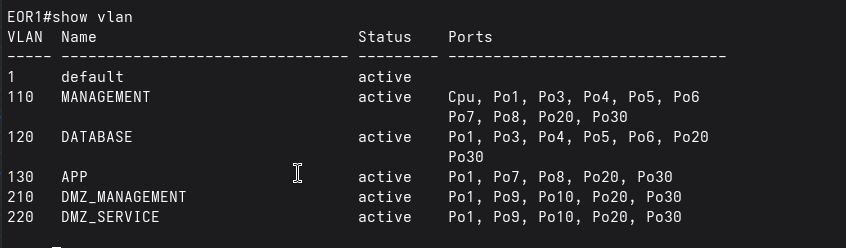
\includegraphics[width=\textwidth,keepaspectratio]{figures/eor1/eor1_vlans.png}
    \caption{EoR-1: VLANs (\texttt{show vlan}).}
    \label{fig:app-eor1-vlans}
\end{figure}

\begin{figure}[H]
    \centering
    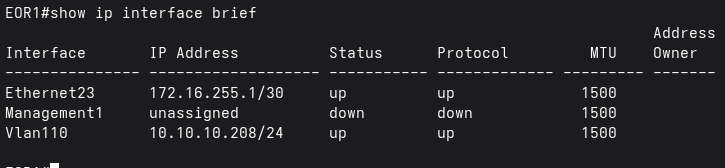
\includegraphics[width=\textwidth,keepaspectratio]{figures/eor1/eor1_ip.png}
    \caption{EoR-1: IP addressing (\texttt{show ip interface brief}).}
    \label{fig:app-eor1-ip}
\end{figure}

\begin{figure}[H]
    \centering
    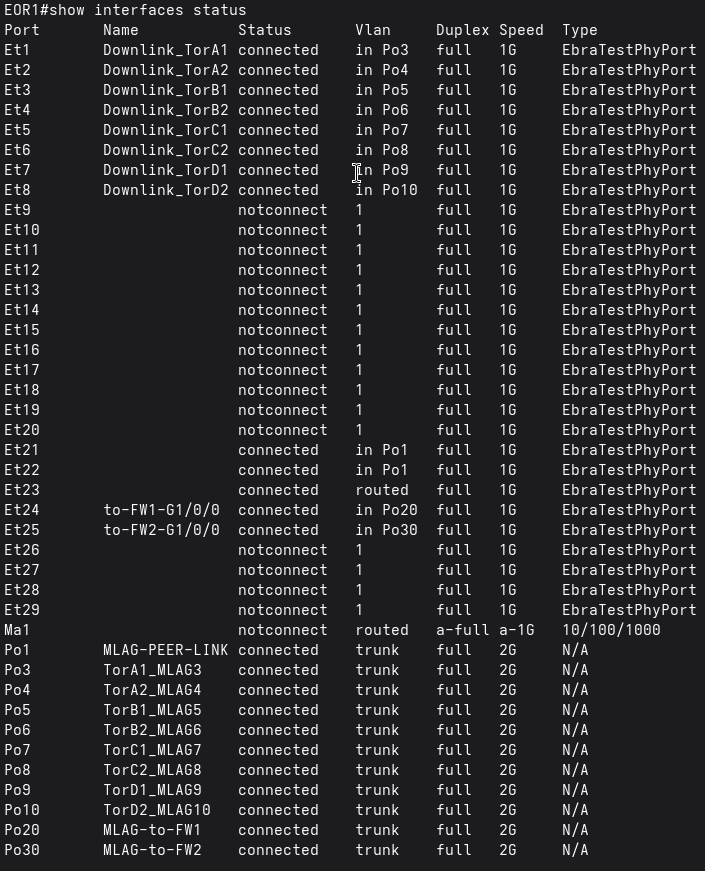
\includegraphics[width=\textwidth,keepaspectratio]{figures/eor1/eor1_interfaces.png}
    \caption{EoR-1: Interfaces and Port-Channels.}
    \label{fig:app-eor1-interfaces}
\end{figure}

\begin{figure}[H]
    \centering
    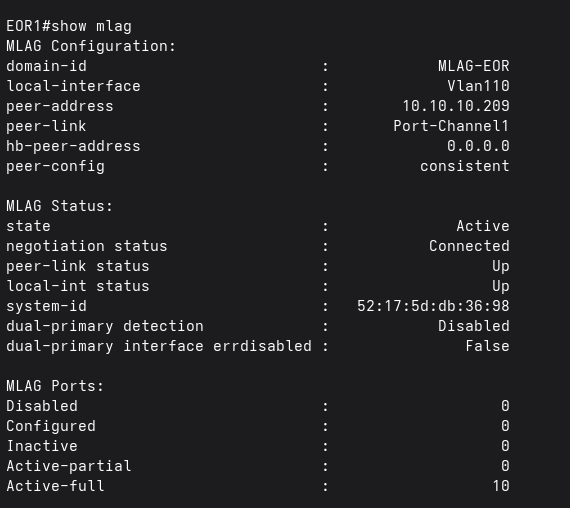
\includegraphics[width=\textwidth,keepaspectratio]{figures/eor1/eor1_mlag_default.png}
    \caption{EoR-1: MLAG (\texttt{show mlag}).}
    \label{fig:app-eor1-mlag}
\end{figure}

\section{ToR A-1 (Arista vEOS)}
\addcontentsline{toc}{section}{E.2 ToR A-1}

\begin{figure}[H]
    \centering
    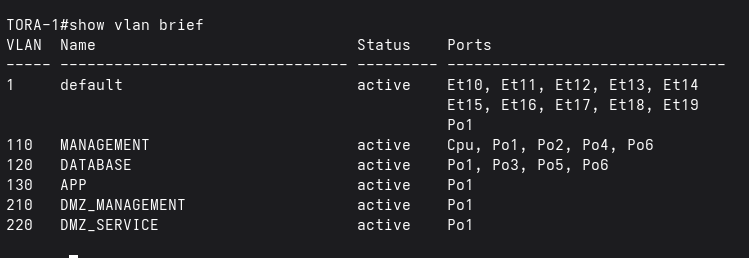
\includegraphics[width=\textwidth,keepaspectratio]{figures/tora1/tora1_vlan.png}
    \caption{ToR A-1: VLANs (\texttt{show vlan brief}).}
    \label{fig:app-tora1-vlans}
\end{figure}

\begin{figure}[H]
    \centering
    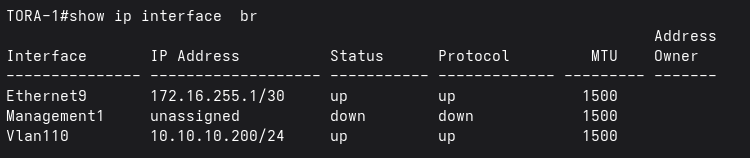
\includegraphics[width=\textwidth,keepaspectratio]{figures/tora1/tora1_ip.png}
    \caption{ToR A-1: IP addressing.}
    \label{fig:app-tora1-ip}
\end{figure}

\begin{figure}[H]
    \centering
    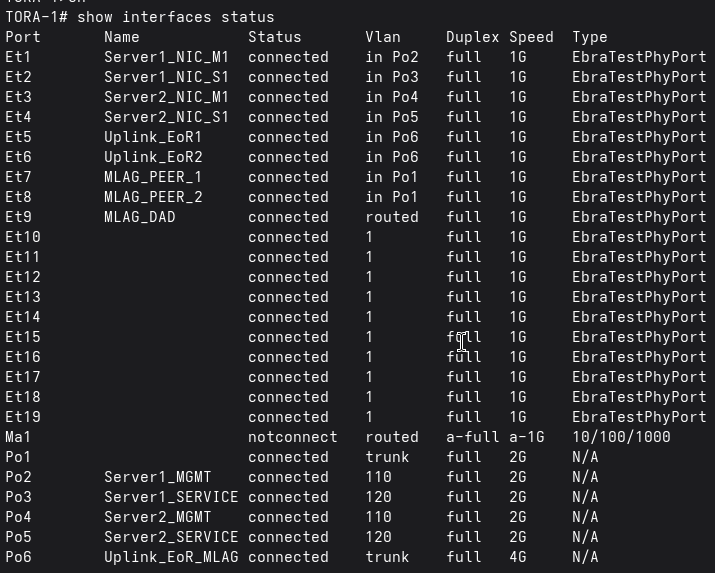
\includegraphics[width=\textwidth,keepaspectratio]{figures/tora1/tora1_interfaces.png}
    \caption{ToR A-1: Interfaces and Port-Channels.}
    \label{fig:app-tora1-interfaces}
\end{figure}

\begin{figure}[H]
    \centering
    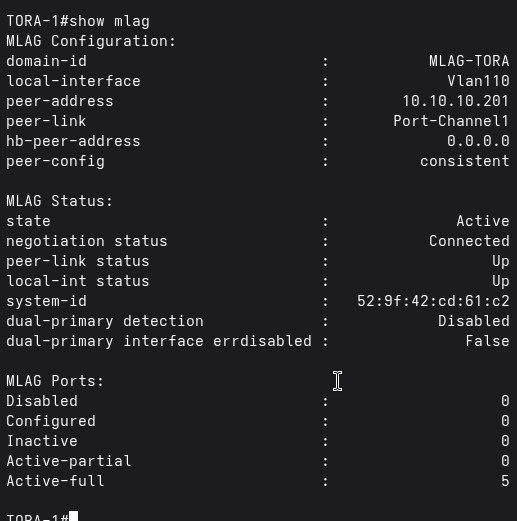
\includegraphics[width=\textwidth,keepaspectratio]{figures/tora1/tora1_mlag_default.png}
    \caption{ToR A-1: MLAG (\texttt{show mlag}).}
    \label{fig:app-tora1-mlag}
\end{figure}

\section{Firewalls (pfSense)}
\addcontentsline{toc}{section}{E.3 Firewalls}

\begin{figure}[H]
    \centering
    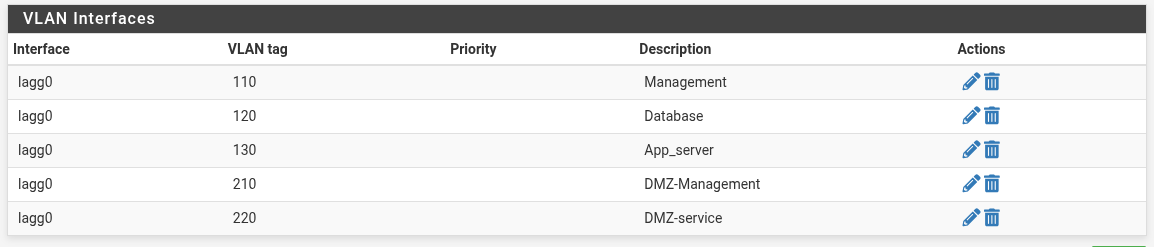
\includegraphics[width=\textwidth,keepaspectratio]{figures/fw1/fw1_vlan.png}
    \caption{FW-1: VLAN interfaces.}
    \label{fig:app-fw1-vlans}
\end{figure}

\begin{figure}[H]
    \centering
    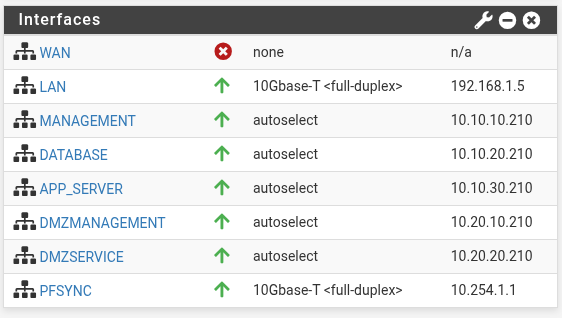
\includegraphics[width=\textwidth,keepaspectratio]{figures/fw1/fw1_interfaces_ips.png}
    \caption{FW-1: Interfaces and IPs.}
    \label{fig:app-fw1-interfaces}
\end{figure}

\begin{figure}[H]
    \centering
    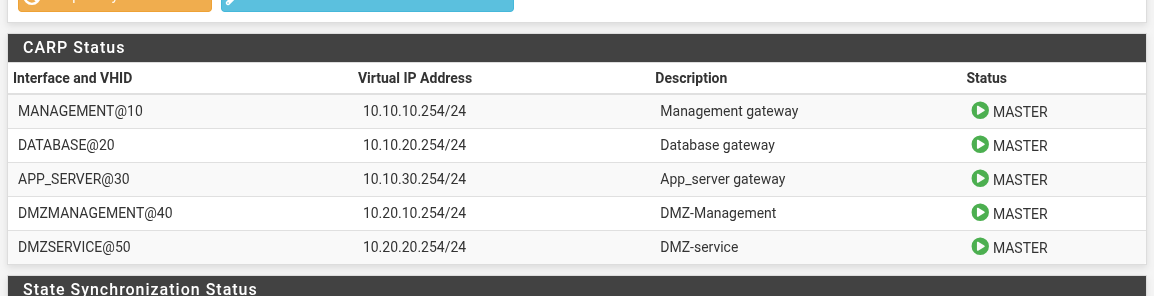
\includegraphics[width=\textwidth,keepaspectratio]{figures/fw1/fw1_vrrp.png}
    \caption{FW-1: CARP (master).}
    \label{fig:app-fw1-vrrp}
\end{figure}

\begin{figure}[H]
    \centering
    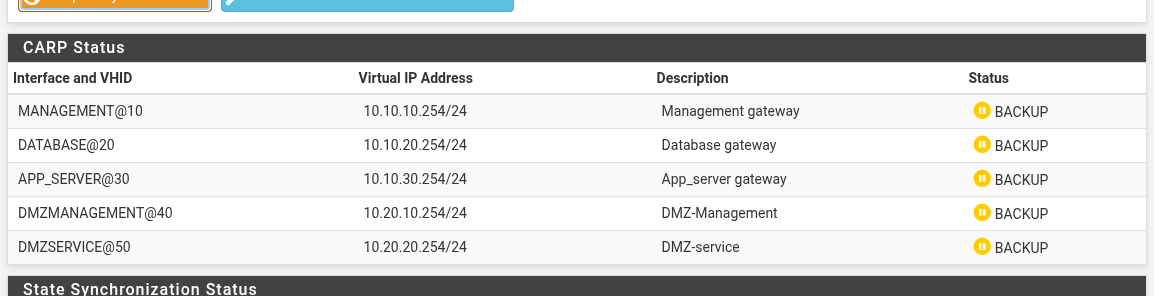
\includegraphics[width=\textwidth,keepaspectratio]{figures/fw1/fw2_vrrp.png}
    \caption{FW-2: CARP (backup).}
    \label{fig:app-fw2-vrrp}
\end{figure}

\begin{figure}[H]
    \centering
    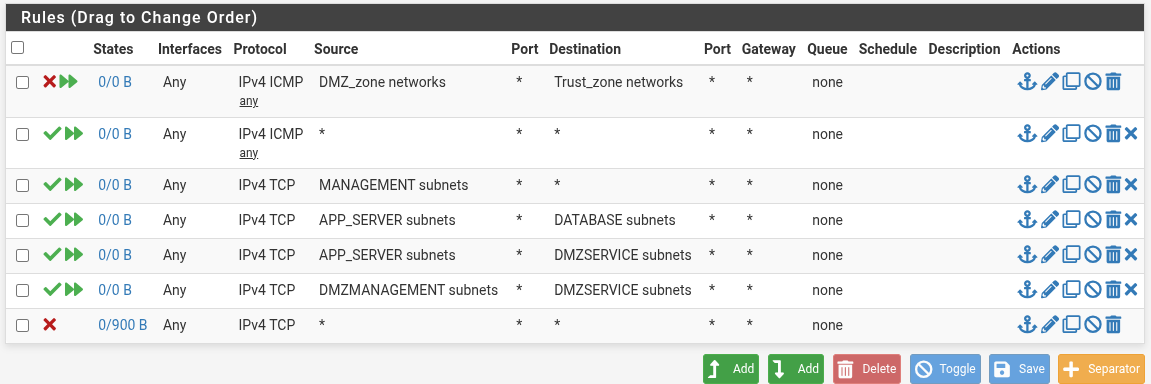
\includegraphics[width=\textwidth,keepaspectratio]{figures/fw1/fw1_rules.png}
    \caption{FW-1: Firewall rules.}
    \label{fig:app-fw1-rules}
\end{figure}

\section{Server 1 (Linux)}
\addcontentsline{toc}{section}{E.4 Server 1}

\begin{figure}[H]
    \centering
    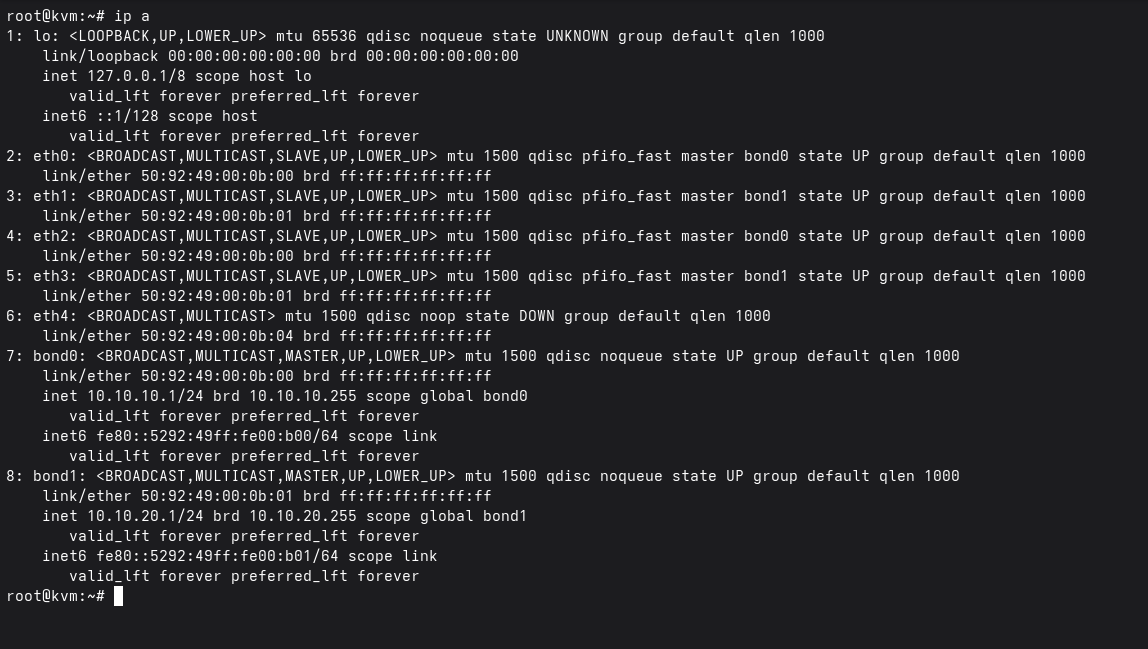
\includegraphics[width=\textwidth,keepaspectratio]{figures/server1/server1_config.png}
    \caption{Server~1: Bonding and IP assignments (\texttt{ip a}).}
    \label{fig:app-server1-config}
\end{figure}
